\chapter{Design Patterns}

Initially proposed by Christopher Alexander in the context of architecture.

\begin{center}
  A reusable \textcolor[HTML]{FF6600}{solution}\\
  to a known \textcolor[HTML]{FF6600}{problem}\\
  in a well defined \textcolor[HTML]{FF6600}{context}\\
\end{center}

The context is a \(design\) situation giving rise to a (design) problem.


The problem is a set of forces repeatedly arising in the context. \footnote{Any relevant aspect of the problem E.g., requirements,
  constraints, desirable properties}

The solution is a proven resolution of the problem. Configuration to balance forces.
Structure with components and relationships and run-time behaviour.

\paragraph{Example of Social Pattern:} You are in queue to the supermarket gastronomic section.
The problem is hard to spot who arrived first. The solution is to use a ticket machine.

\section{Types of Software Patterns}

\begin{itemize}
  \item \textbf{Architectural patterns} - high level structures of software systems. E.g., layered architecture, client-server, microservices.
  \item \textbf{Design patterns} - solutions to common design problems. E.g., Singleton, Observer, Factory Method.
  \item \textbf{Idioms} - language-specific patterns. E.g., RAII in C++, list comprehensions in Python.
\end{itemize}

\subsection{Architectural pattern}
Normally the architectural pattern works with big components and their interactions and is needed to describe the responsibilities of these components.
Expresses a fundamental structural organization schema for software systems and defines the rules and guidelines for organizing the
relationships between the components.

\paragraph{Example of architectural pattern:} Several programs that are used in sequence read from
input and write sequentially to output.

The problem is there are a lot of intermediate files used for
communication between programs.

The solution is to adopt pipes and filters architecture feeding with the result of the previous one.

\subsection{Design patterns}

Provides a scheme for refining components of a software system or their relationships and describes a commonly recurring structure of
communicating components.

\paragraph{Example of design pattern:} A class library providing few functionalities contains a
lot of classes.

The problem is the user is exposed to the internal complexity of the library.

The solution is to create a new façade class that interacts with the user
and hide all the details.

\subsection{Idioms}

It is a low-level pattern specific to a programming
language. Describes how to implement particular aspects of
components or the relationships between them.
Leverages the features of a programming
language.

\paragraph{Example of idioms:} An attribute is constant and should be globally
available to many classes.

The problem is opening access would allow unauthorized
modifications and the attribute is repeated in every object.

The solution is to make public static final in Java language.

\section{Pattern language}

Pattern do not exist in isolation in fact can happen that two or more patterns are applied together,
used to implement part of another pattern and introduce a problem solved by another

They are called Pattern Languages or pattern systems.\newline


\noindent\begin{minipage}{0.95\linewidth}
  % Primo blocco: 50% dello spazio per il codice
  \begin{minipage}[t]{0.5\linewidth}

    Collection of patterns together with guidelines for:

    \begin{itemize}
      \item Implementation
      \item Combination
      \item Practical use
    \end{itemize}


  \end{minipage}% <-- IMPORTANTE: il simbolo % qui evita spazi bianchi extra
  \hfill
  \begin{minipage}[t]{0.47\linewidth}


    Should:

    \begin{itemize}
      \item Count enough patterns
      \item Describe patterns uniformly
      \item Present relationships
    \end{itemize}

  \end{minipage}
\end{minipage}

\section{Idioms}

\subsubsection{X-ability}
Clonability, serializability, comparability, etc. some specific
behaviour dealing with many heterogeneous classes.
The solution is to derive from a class or interface that defines the
required methods.

\paragraph{Example:} In Java all methods extends the root class \textit{Object}
and provides the methods \textit{toString()}, \textit{equals()}, \textit{hashCode()}, etc. that can be overridden to provide specific behaviour.

\subsection{Strong typing vs. Duck Typing}

\textit{"If it looks like a duck, swims like a duck, and quacks like a duck, then it probably is a duck."}

\textbf{Strong typed language:} You must define interfaces and classes to be able to
call a specific method. Compile time type checking.

\textbf{Dynamic/duck typed language:} You just add a method to a class and you can call it.
No compile time type checking.

\subsection{Property}
A property, more general than an attribute, is a named characteristic of an object typically accessed through well-defined operations
called accessors, getters, and setters forming the public interface of the object and it is not
necessarily an attribute of the object (e.g. the age can be derived from the date of birth).

\section{Design Patterns}
Description of communicating objects and classes
that are customized to solve a general design
problem in a particular context.

A design pattern names, abstracts, and identifies
the key aspects of a common design structure
that make it useful for creating a reusable object-
oriented design.

\begin{table}[h!]
  \centering
  \renewcommand{\arraystretch}{1.8}
  \begin{tabular}{ccccc}
                                                    &        & \multicolumn{3}{c}{\textbf{Purpose}}                           \\
    \hline
                                                    &        & Creational                           & Structural & Behavioral \\
    \hline
    \multirow{2}{*}{\rotatebox{90}{\textbf{Scope}}} & Class  & 1                                    & 1          & 2          \\
                                                    & Object & 4                                    & 6          & 10         \\
    \hline
  \end{tabular}
\end{table}

\paragraph{Pattern selection}
How to use patterns? First of all you need to know the problem you
are trying to solve, knowing the patterns and then select the one that
best fits your needs.

\subsection{Creational patterns}

\vspace{0.5cm}
\noindent\begin{minipage}{\linewidth}
  \begin{minipage}[t]{0.35\linewidth}
    \begin{itemize}
      \item \textbf{Class}: Factory Method
    \end{itemize}
  \end{minipage}%
  \hfill
  \begin{minipage}[t]{0.65\linewidth}
    \begin{itemize}
      \item \textbf{Object}: Abstract Factory, Builder, Prototype, Singleton

    \end{itemize}
  \end{minipage}
\end{minipage}

\subsubsection{Abstract Factory}



\begin{center}
  \centering
  \begin{minipage}{\linewidth}
    % Primo blocco: 50% dello spazio per il codice
    \begin{minipage}{0.7\linewidth}

      A family of related classes can have different
      implementation details.

      The client should not know anything about which
      variant they are using / creating.

      \paragraph{Example:} GUI where you have different components (buttons, text fields, etc.) and the same
      GUI can be applied to different platforms such as Windows, MacOS, Linux, etc.

    \end{minipage}% <-- IMPORTANTE: il simbolo % qui evita spazi bianchi extra
    \hfill
    \begin{minipage}{0.3\linewidth}

      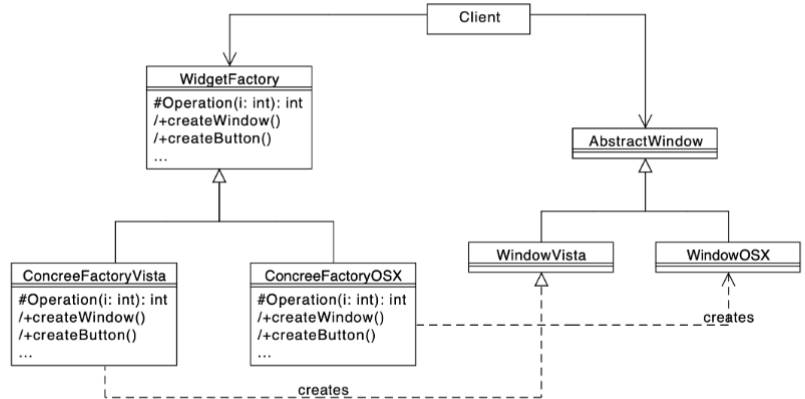
\includegraphics[width=\linewidth]{images/DesignPatterns/DP-esempio1.png}

    \end{minipage}
  \end{minipage}
\end{center}


\subsubsection{Singleton}

\begin{center}
  \centering
  \begin{minipage}{\linewidth}
    % Primo blocco: 50% dello spazio per il codice
    \begin{minipage}{0.7\linewidth}

      A class represents a concept that requires a single
      instance.

      The client should be able to access, in approper way, the unique instance.\newline

      \noindent
      \begin{tcolorbox}
        \textbf{Note:} If we talk about of an object designer pattern, in python you can
        just create a global variable and it will be a singleton.
      \end{tcolorbox}
    \end{minipage}% <-- IMPORTANTE: il simbolo % qui evita spazi bianchi extra
    \hfill
    \begin{minipage}{0.3\linewidth}

      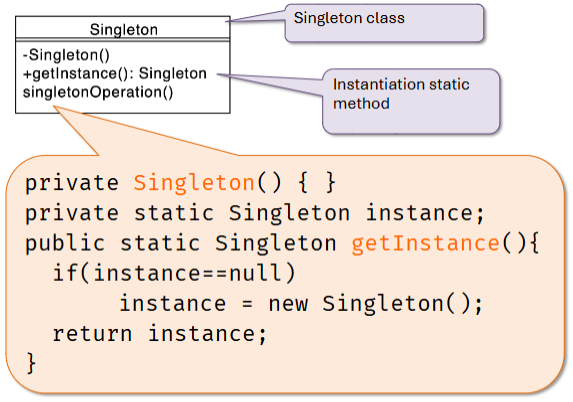
\includegraphics[width=\linewidth]{images/DesignPatterns/DP-esempio2.png}

    \end{minipage}
  \end{minipage}
\end{center}


\subsubsection{Builder}

\begin{center}
  \centering
  \begin{minipage}{\linewidth}
    % Primo blocco: 50% dello spazio per il codice
    \begin{minipage}{0.7\linewidth}

      An object of a complex class has to be created.

      The creation entails complex interaction with the
      object and could be different variations of the object.

    \end{minipage}% <-- IMPORTANTE: il simbolo % qui evita spazi bianchi extra
    \hfill
    \begin{minipage}{0.3\linewidth}

      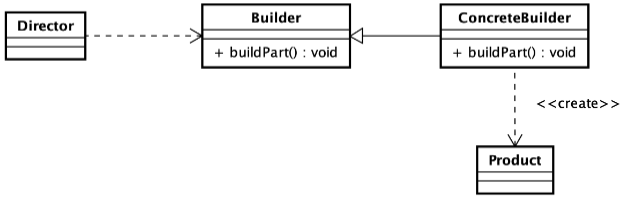
\includegraphics[width=\linewidth]{images/DesignPatterns/DP-esempio3.png}

    \end{minipage}
  \end{minipage}
\end{center}

\paragraph{Example:} $10.40\,kg\cdot m^2\cdot s^{-3}$

\begin{center}
  \centering
  \begin{minipage}{\linewidth}
    % Primo blocco: 50% dello spazio per il codice
    \begin{minipage}[t]{0.47\linewidth}

      \begin{minted}[breaklines]{java}
//Usual non-fluent builder
Measure power = new Measure(10.4);
power.addUnit("kg", 1);
power.addUnit("m", 2);
power.addUnit("s", -3);
power.setPrecision(2);
\end{minted}

    \end{minipage}% <-- IMPORTANTE: il simbolo % qui evita spazi bianchi extra
    \hfill
    \begin{minipage}[t]{0.47\linewidth}

      \begin{minted}{java}
//Fluent builder
Measure power = new Measure.Builder(10.4)
    .is("kg").by("m")
    .squared().by("s").to(-3)
    .withPrecision(2).build();
\end{minted}

    \end{minipage}
  \end{minipage}
\end{center}

\subsubsection{Prototype}



\begin{center}
  \centering
  \begin{minipage}{\linewidth}
    % Primo blocco: 50% dello spazio per il codice
    \begin{minipage}{0.7\linewidth}
      Several object can be created out of a palette of
      similar classes.

      The class hierarchy can become quite complex and
      classes in hierarchy are differentiated by minor
      parameters (that could be defined through
      constructor arguments).

      A solution could be start with a prototype classe and
      clone it to create new objects.


      \paragraph{Example:} A graphical editor where you
      have very similar shapes (e.g. square with different radius, colors, etc.).


    \end{minipage}% <-- IMPORTANTE: il simbolo % qui evita spazi bianchi extra
    \hfill
    \begin{minipage}{0.3\linewidth}

      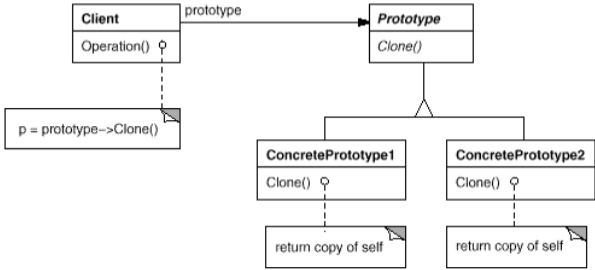
\includegraphics[width=\linewidth]{images/DesignPatterns/DP-esempio4.png}

    \end{minipage}
  \end{minipage}
\end{center}


\subsection{Structural patterns}

How  organize classes and objects to compose larger structures.

\vspace{0.5cm}
\noindent\begin{minipage}{\linewidth}
  \begin{minipage}[t]{0.35\linewidth}
    \begin{itemize}
      \item \textbf{Class}: Adapter
    \end{itemize}
  \end{minipage}%
  \hfill
  \begin{minipage}[t]{0.65\linewidth}
    \begin{itemize}
      \item \textbf{Object}: Bridge, Composite, Decorator, Facade, Flyweight, Proxy

    \end{itemize}
  \end{minipage}
\end{minipage}

\subsubsection{Adapter}


\begin{center}
  \centering
  \begin{minipage}{\linewidth}
    % Primo blocco: 50% dello spazio per il codice
    \begin{minipage}{0.7\linewidth}

      A class provides the features required by another
      class but its interface is not the one expected by the client.

      The integration of the provider class should be
      possible without modifying it. The source code could be not available
      or is already used as it is somewhere else.

      \paragraph{Example:} In Java, keyboard events are handled by
      KeyListener. Listener class need to implement the interface
      and implement all the methods. If you are interested only
      in one of the methods, you can use the KeyAdapter class
      that is empty and you can decide which method to override,
      and the Listener extends KeyAdapter instead of KeyListener.

    \end{minipage}% <-- IMPORTANTE: il simbolo % qui evita spazi bianchi extra
    \hfill
    \begin{minipage}{0.3\linewidth}

      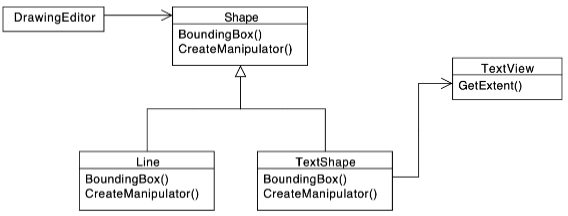
\includegraphics[width=\linewidth]{images/DesignPatterns/DP-esempio5.png}

    \end{minipage}
  \end{minipage}
\end{center}


\subsubsection{Composite}


\begin{center}
  \centering
  \begin{minipage}{\linewidth}
    % Primo blocco: 50% dello spazio per il codice
    \begin{minipage}{0.7\linewidth}

      You need to represent part-whole hierarchies of
      objects.

      Clients can be very complex and they require
      to adapt the difference between all the elements
      in the hierarchy.

      \paragraph{Example:} In Java UI components are organized
      in a tree structure. You can have a panel that contains
      other panels and buttons, etc.

    \end{minipage}% <-- IMPORTANTE: il simbolo % qui evita spazi bianchi extra
    \hfill
    \begin{minipage}{0.3\linewidth}

      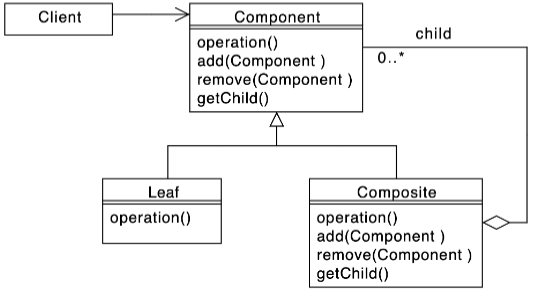
\includegraphics[width=\linewidth]{images/DesignPatterns/DP-esempio6.png}

    \end{minipage}
  \end{minipage}
\end{center}



\subsubsection{Decorator}


\begin{center}
  \centering
  \begin{minipage}{\linewidth}
    % Primo blocco: 50% dello spazio per il codice
    \begin{minipage}{0.7\linewidth}

      You have some objects of classes that have
      specific behaviour and you want to add the same
      behaviour plus someting else dynamically.

      The solution can be extend the class but
      if that behaviour is something you would to apply
      to many classes, you need to extend all of leaf classes.
      Using a decorator you can modyfy the behaviour
      without creating an explosion
      of subclasses for every combination of features

      \paragraph{Example:} In Java we have JScrollPane can
      be used to provide a scroll pane to
      any component


    \end{minipage}% <-- IMPORTANTE: il simbolo % qui evita spazi bianchi extra
    \hfill
    \begin{minipage}{0.3\linewidth}

      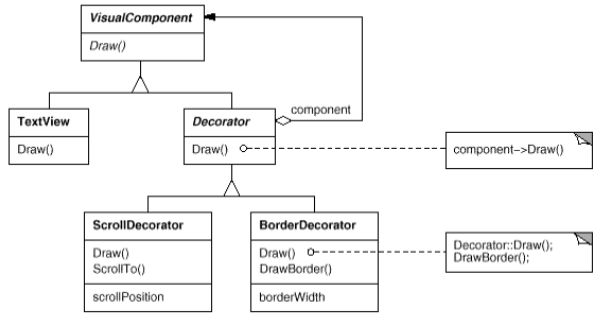
\includegraphics[width=\linewidth]{images/DesignPatterns/DP-esempio7.png}

    \end{minipage}
  \end{minipage}
\end{center}


\subsubsection{Flyweight}


\begin{center}
  \centering
  \begin{minipage}{\linewidth}
    % Primo blocco: 50% dello spazio per il codice
    \begin{minipage}{0.7\linewidth}

      You need need to create a very large number of similar
      objects, and memory usage and performance become concerns.

      \paragraph{Example:} In Java we can pool different objects
      togheter. The Integer class in Java.

    \end{minipage}% <-- IMPORTANTE: il simbolo % qui evita spazi bianchi extra
    \hfill
    \begin{minipage}{0.3\linewidth}

      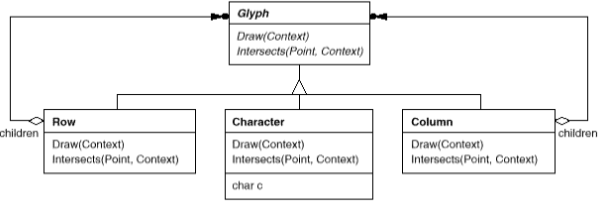
\includegraphics[width=\linewidth]{images/DesignPatterns/DP-esempio8.png}

    \end{minipage}
  \end{minipage}
\end{center}



\subsubsection{Proxy}

You need to controll access to an object.

We need to provide a placeholder that is able to
mediate between the client needs and all the requirements
you want to controll before accessing the final object without
changing interface or class.

\begin{itemize}
  \item \textbf{Remote proxy}: provides a local representative for an
        object in a different address space.
  \item \textbf{Virtual proxy}: creates expensive objects on demand. E.g.
        slow loading resource - images in a web page.
  \item \textbf{Protection proxy}: controls access to the original object.
        E.g. when objects should have different access rights.
  \item \textbf{Smart reference}: is a replacement for a bare pointer that
        performs additional actions when an object is accessed. E.g. counting the number of references, checking permissions, etc.
\end{itemize}

\subsubsection{Facade}


\begin{center}
  \centering
  \begin{minipage}{\linewidth}
    % Primo blocco: 50% dello spazio per il codice
    \begin{minipage}{0.7\linewidth}

      Hide the details and the complexity of a general class by providing
      a simpler interface.
      The client should not know anything about the subsystem.

    \end{minipage}% <-- IMPORTANTE: il simbolo % qui evita spazi bianchi extra
    \hfill
    \begin{minipage}{0.3\linewidth}

      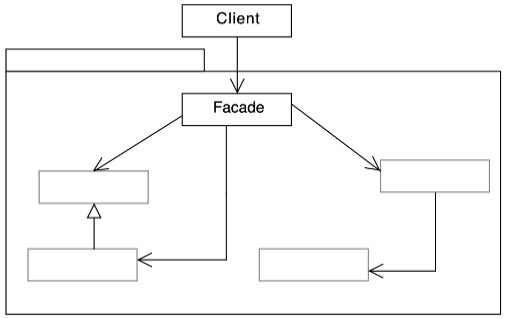
\includegraphics[width=0.75\linewidth]{images/DesignPatterns/DP-esempio9.png}

    \end{minipage}
  \end{minipage}
\end{center}

\subsection{Behavioral patterns}
Behavioral patterns allow to implement specific algorithms
using objects and classes to provide control and flexibility.

\vspace{0.5cm}
\noindent\begin{minipage}{\linewidth}
  \begin{minipage}[t]{0.35\linewidth}
    \begin{itemize}
      \item \textbf{Class}: Interpreter, Template Method
    \end{itemize}
  \end{minipage}%
  \hfill
  \begin{minipage}[t]{0.65\linewidth}
    \begin{itemize}
      \item \textbf{Object}: Chain of Responsibility, Command, Iterator, Mediator, Memento, Observer, State, Strategy, Visitor
    \end{itemize}
  \end{minipage}
\end{minipage}
\vspace{0.5cm}

The basic mechanism of behavioral patterns is enapsultion variation.
Instead of having a lot of if-else you have a structure at object level
that allows you to define different alternatives.

\subsection{Template Method}

\begin{center}
  \centering
  \begin{minipage}{\linewidth}
    \begin{minipage}{0.7\linewidth}

      An algorithm/behavior has a stable core and several
      variation at given points. You have to implement/maintain several almost
      identical pieces of code.

      \paragraph{Example:} The compare in Java. You have to implement the compare method that solves integer or string comparison.

    \end{minipage}% <-- IMPORTANTE: il simbolo % qui evita spazi bianchi extra
    \hfill
    \begin{minipage}{0.3\linewidth}

      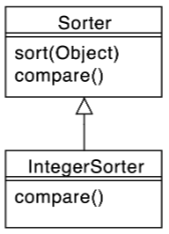
\includegraphics[width=0.3\linewidth]{images/DesignPatterns/DP-esempio10.png}

    \end{minipage}
  \end{minipage}
\end{center}


\subsection{Strategy Pattern}

% \begin{flushleft}
%   \raggedright
%   \begin{minipage}{\linewidth}
%     \begin{minipage}{0.7\linewidth}

%       Many classes or algorithm has a stable core and
%       several behavioral variations, several different
%       implementations are needed.
%       Every variation of an algorithm can be embedded
%       in an object and passed as a parameter to
%       the algorithm.

%       \paragraph{Example:} Comparator in Java.

%       Consequences:

%       \begin{itemize}
%         \item [+] Avoid conditional statements
%         \item [+] Algorithms may be organized in families
%         \item [+] Choice of implementations
%         \item [+] Run-time binding
%         \item [-] Clients must be aware of different strategies
%         \item [-] Communication overhead
%         \item [-] Increased number of objects
%       \end{itemize}

%     \end{minipage}% <-- IMPORTANTE: il simbolo % qui evita spazi bianchi extra
%     \hfill
%     \begin{minipage}{0.3\linewidth}

%       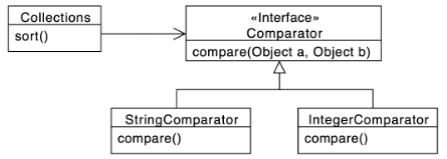
\includegraphics[width=\linewidth]{images/DesignPatterns/DP-esempio11.png}

%     \end{minipage}
%   \end{minipage}
% \end{flushleft}

\begin{flushleft}
  \begin{minipage}{0.96\linewidth}
    \begin{minipage}[c]{0.37\linewidth}
      Many classes or algorithm has a stable core and
      several behavioral variations, several different
      implementations are needed.


      Every variation of an algorithm can be embedded
      in an object and passed as a parameter to
      the algorithm.

      \paragraph{Example:} Comparator in Java.



    \end{minipage}%
    \hfill
    \begin{minipage}[c]{0.37\linewidth}
      \centering
      \textbf{Consequences}:

      \begin{itemize}
        \item [+] Avoid conditional statements
        \item [+] Algorithms may be organized in families
        \item [+] Choice of implementations
        \item [+] Run-time binding
        \item [-] Clients must be aware of different strategies
        \item [-] Communication overhead
        \item [-] Increased number of objects
      \end{itemize}
    \end{minipage}%
    \hfill
    \begin{minipage}[c]{0.25\linewidth}
      \centering
      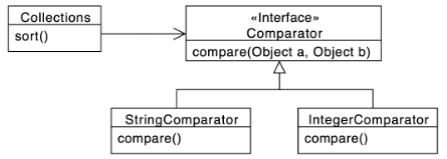
\includegraphics[width=\linewidth]{images/DesignPatterns/DP-esempio11.png}
    \end{minipage}
  \end{minipage}
\end{flushleft}


\subsection{Iterator pattern}

\begin{center}
  \centering
  \begin{minipage}{\linewidth}
    \begin{minipage}{0.7\linewidth}

      You have a collection of objects and you want to iterate
      on it allowing multiple concurrent iterators.

      \paragraph{Example:} In Java there is the Iterable interface and Iterator.

    \end{minipage}% <-- IMPORTANTE: il simbolo % qui evita spazi bianchi extra
    \hfill
    \begin{minipage}{0.27\linewidth}

      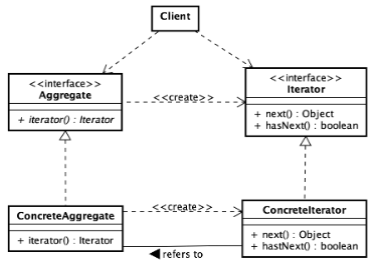
\includegraphics[width=\linewidth]{images/DesignPatterns/DP-esempio12.png}

    \end{minipage}
  \end{minipage}
\end{center}

\subsection{Observer pattern}

\begin{flushleft}
  \raggedright
  \begin{minipage}{\linewidth}
    \begin{minipage}{0.7\linewidth}

      The change in one object may influence one or more
      other objects. This can cause high coupling between objects
      and the number and type of objects to be notified may not be
      known in advance.

      \paragraph{Example:} In Java there is the Observable interface and Observer interface. This is very common in UI programming.

      Consequences:

      \begin{itemize}
        \item [+] Abstract coupling between Subject and Observer
        \item [+] Support for broadcast communication
        \item [-] Unanticipated updates
      \end{itemize}

    \end{minipage}% <-- IMPORTANTE: il simbolo % qui evita spazi bianchi extra
    \hfill
    \begin{minipage}{0.3\linewidth}

      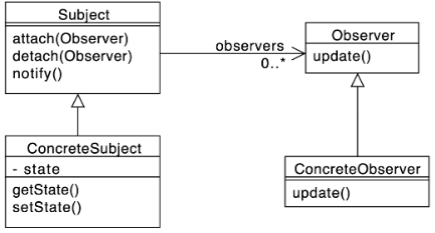
\includegraphics[width=\linewidth]{images/DesignPatterns/DP-esempio13.png}

    \end{minipage}
  \end{minipage}
\end{flushleft}

\subsection{Visitor}

\begin{center}
  \centering
  \begin{minipage}{\linewidth}
    \begin{minipage}{0.7\linewidth}

      You have an object structure that contains many classes
      with different interfaces and you want to perform
      several different and unrelated operations on these objects.

      The operations depend on the concrete classes and
      you want to avoid putting many different methods in each of
      these classes.

    \end{minipage}% <-- IMPORTANTE: il simbolo % qui evita spazi bianchi extra
    \hfill
    \begin{minipage}{0.3\linewidth}

      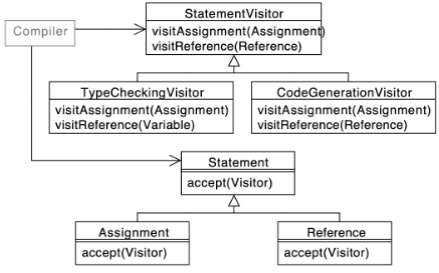
\includegraphics[width=\linewidth]{images/DesignPatterns/DP-esempio14.png}

    \end{minipage}
  \end{minipage}
\end{center}

\section{Inheritance vs. composition}


\begin{flushleft}
  \raggedright

  \begin{minipage}{\linewidth}
    \begin{minipage}{0.7\linewidth}
      Reuse can be achieved via:

      \begin{itemize}
        \item \textbf{Inheritance}: a new class is created by
              inheriting from an existing class and adding new features
              or modifying existing ones. Clients can invoke directly
              inherited methods.

        \item \textbf{Composition}: The class has a link or
              instance to a class you want to reuse and just forwards
              the calls to it.
      \end{itemize}

      \begin{tcolorbox}
        \textbf{Note:} The Observable pattern is deprecated. The PropertyChangeSupport is more flexible.
      \end{tcolorbox}

    \end{minipage}% <-- IMPORTANTE: il simbolo % qui evita spazi bianchi extra
    \hfill
    \begin{minipage}{0.3\linewidth}

      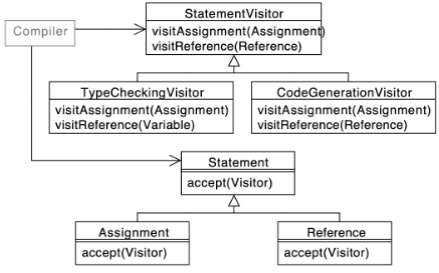
\includegraphics[width=\linewidth]{images/DesignPatterns/DP-esempio14.png}

    \end{minipage}
  \end{minipage}
\end{flushleft}


\section{Abstract Syntax Tree}

The AST is a tree that represent a syntax of formal language.
We can use the composite pattern to representationt he arithmetic expressions.

And using the visitor pattern or the interpreter pattern to evaluate the expression.

\section{Model View Controller}


% \begin{center}
%   \begin{minipage}{0.96\linewidth}
%     \begin{minipage}[t]{0.47\linewidth}
%       \textbf{Context}: Interactive applications with flexible HCI.

%       \textbf{Problem}: The same information is presented in different ways/windows, Windows must present consistent data, Should be possible to add/change presentations of information

%     \end{minipage}%
%     \hfill
%     \begin{minipage}[t]{0.25\linewidth}

%       \centering
%       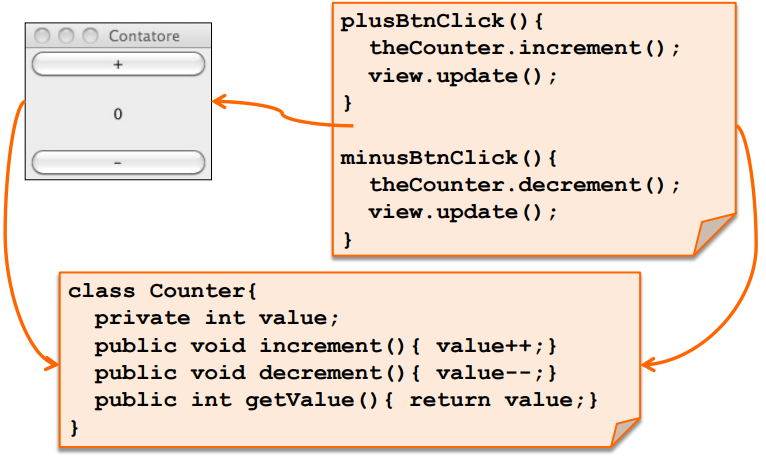
\includegraphics[width=\linewidth]{content/chapters/images/2026-05-23-13-56-44.png}


%     \end{minipage}%
%     \hfill
%     \begin{minipage}[t]{0.25\linewidth}

%       \centering
%       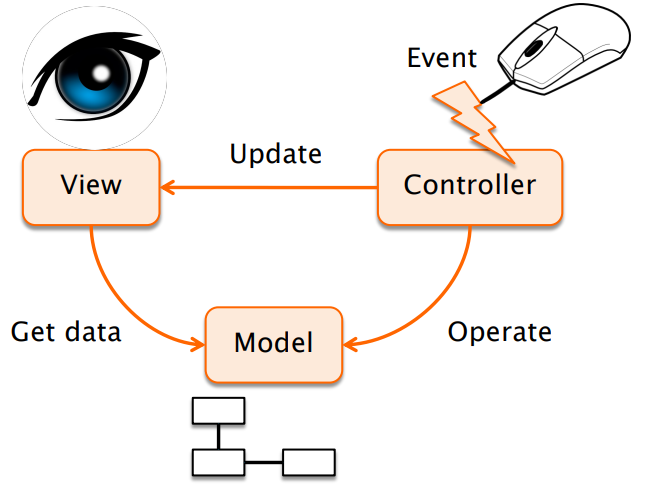
\includegraphics[width=\linewidth]{content/chapters/images/2026-05-23-13-57-10.png}

%     \end{minipage}
%   \end{minipage}
% \end{center}


\begin{center}
  \begin{minipage}{0.96\linewidth}
    \begin{minipage}[c]{0.47\linewidth}
      \textbf{Context}: Interactive applications with flexible HCI.

      \textbf{Problem}: The same information is presented in different ways/windows, Windows must present consistent data, Should be possible to add/change presentations of information
    \end{minipage}%
    \hfill
    \begin{minipage}[c]{0.25\linewidth}
      \centering
      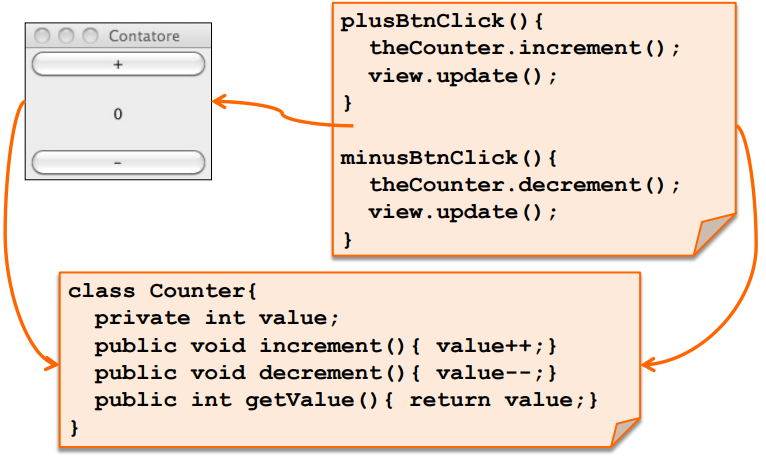
\includegraphics[width=0.9\linewidth]{content/chapters/images/2026-05-23-13-56-44.png}
    \end{minipage}%
    \hfill
    \begin{minipage}[c]{0.25\linewidth}
      \centering
      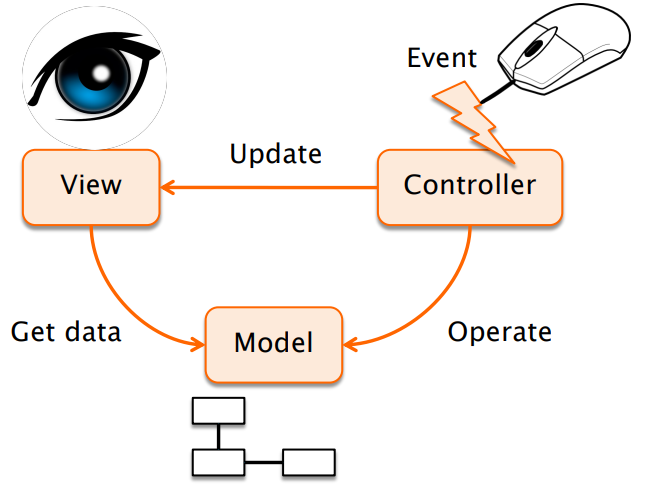
\includegraphics[width=0.9\linewidth]{content/chapters/images/2026-05-23-13-57-10.png}
    \end{minipage}
  \end{minipage}
\end{center}

\subsection{MVC Principles}


When building a GUI we must consider two main
aspects:


\begin{itemize}
  \item Layout (\textbf{View}): how to place the graphical elements to achieve a give visual aspect
  \item Events (\textbf{Controller}): which behavior associate to elements' events
  \item Application logic (\textbf{Model}):  must remain, as far as possible, separate from user interface.
\end{itemize}

\begin{center}
  \begin{minipage}[t]{0.5\linewidth}
    \begin{minipage}[t]{0.45\linewidth}

      \centering
      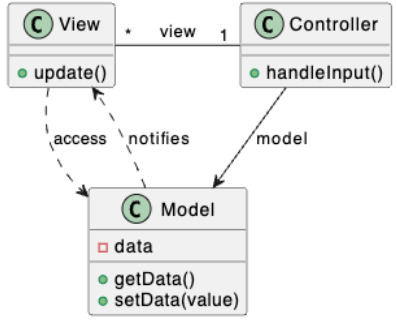
\includegraphics[width=0.7\linewidth]{content/chapters/images/2026-05-23-14-00-23.png}
      \captionof{figure}{MVC}

      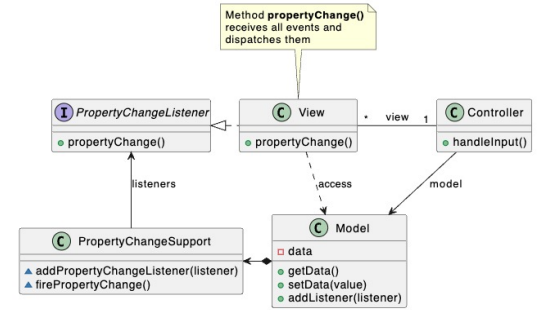
\includegraphics[width=\linewidth]{content/chapters/images/2026-05-23-14-05-32.png}

    \end{minipage}%
    \hfill
    \begin{minipage}[t]{0.45\linewidth}
      \centering
      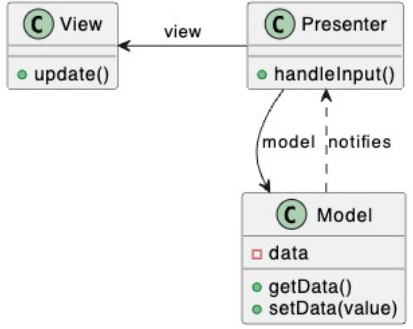
\includegraphics[width=0.7\linewidth]{content/chapters/images/2026-05-23-14-00-48.png}
      \captionof{figure}{MVP}
      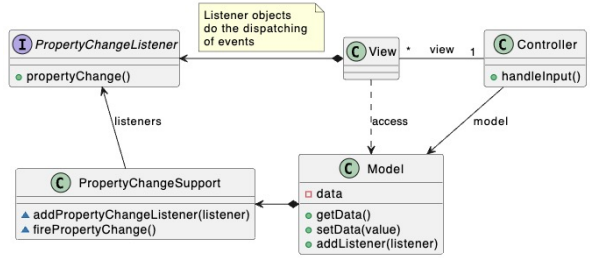
\includegraphics[width=\linewidth]{content/chapters/images/2026-05-23-14-05-59.png}
    \end{minipage}
  \end{minipage}
\end{center}


\subsection{Execution flow}

There is no predefined order of execution. Operation are performed in response to external
events (e.g. mouse click). Event handling is serialized. To execute operations in parallel threads must be
used. Method main in GUIs has the only goal of instantiating the graphical elements

\section{Summary}

Architectural patterns deal with overall system
structure. They provide a unique metaphor for the system
(e.g. pipe and filters). They address specific domains (e.g. distribution or
interaction) and system evolvability



